\documentclass[runningheads]{llncs}
\usepackage[UTF8,scheme=plain]{ctex}
\usepackage{amsmath,amssymb,booktabs,multirow,graphicx,xcolor,hyperref,array}
\usepackage{caption}
\usepackage{float}
\usepackage{tikz}
\usetikzlibrary{arrows.meta,positioning,fit,calc,backgrounds}
\usepackage{enumitem}
\setlist{nosep,leftmargin=2em}
% 将 Markdown 风格反引号转换为等宽文本，并保护文件名中的下划线。
\catcode`\`=\active
\def`#1`{\texttt{\detokenize{#1}}}
\graphicspath{{figures/}}
\hypersetup{colorlinks=true,linkcolor=blue,urlcolor=blue,citecolor=blue}
% 图注独立于正文排版，便于快速辨识编号与说明。
\renewcommand{\figurename}{Figure}
\captionsetup[figure]{font=small,labelfont=bf,labelsep=period,
  justification=raggedright,singlelinecheck=false,skip=6pt}
\captionsetup{hypcap=false}
% 放宽浮动体的排版边界，避免短图表被单独推到空白浮动页。
\renewcommand{\topfraction}{0.92}
\renewcommand{\bottomfraction}{0.88}
\renewcommand{\textfraction}{0.08}
\renewcommand{\floatpagefraction}{0.72}
\setlength{\textfloatsep}{12pt plus 3pt minus 3pt}
\setlength{\floatsep}{10pt plus 3pt minus 3pt}
\makeatletter
\setlength{\@fptop}{0pt}
\setlength{\@fpsep}{12pt}
\setlength{\@fpbot}{0pt plus 1fil}
\makeatother
\setlength{\emergencystretch}{2em}

\newcommand{\method}{M1}
\newcommand{\full}{FullSchema}
\newcommand{\schemarag}{SchemaRAG}

\title{面向文化遗产记录抽取的预算感知动态 Schema 选择与可扩展 LLM 预处理框架}
\titlerunning{Budget-Aware Dynamic Schema Selection and Scalable LLM Preprocessing}
\author{作者信息待补}
\authorrunning{作者信息待补}
\institute{单位信息待补}

\begin{document}
\maketitle

\begin{abstract}
异构文化遗产记录的信息密度和可抽取字段并不均匀，但对每条记录使用完整 Schema
会引入大量无效字段负载。尚不清楚的是，少量监督能否在不显著损害字段级抽取质量的
情况下支持记录级 Schema 裁剪，并将负载下降传递到端到端流水线。我们利用完整 Schema
抽取产生的模型辅助银标监督，训练字段存在性和输出长度预测器，再结合字段价值先验
与调用前的估计字段成本，在记录级构造预算约束的动态 Schema。使用 100 条独立银标记录
启动训练后，在与训练和验证数据隔离的 500 条冻结评估记录上，Qwen3-8B-AWQ 模型服务在
估计字段成本容量为 200 的配置下达到 Presence Macro-F1 0.7644、Micro-F1 0.7673 和
平均总 Token 385.5。相较当前 SchemaRAG 外部适配实现的固定 Top-10 检索，本方法同时
获得更高的字段一致性与更低的平均 Token；该比较限于当前 embedding 模型和 Top-$k$ 配置。
独立的 2,000 条性能负载实验进一步表明，在使用 16 个并发消费者和
容量为 16 的有界队列时，相比完整 Schema，动态字段选择使在线流水线时间降低 48.54\%，
有效吞吐提高 94.38\%，总 Token 减少 37.44\%。这些结果表明，在当前数据、模型服务
和单进程异步流水线条件下，记录级 Schema 选择具有改善大语言模型（large language
model，LLM）预处理负载的潜力。当前结果受模型辅助银标参照和在线实验边界限制，完整生命周期
成本以及多进程或多节点扩展仍需在其他系统条件下验证。
\end{abstract}

\keywords{文化遗产抽取 \and 动态 Schema \and 大语言模型 \and 预算约束 \and 数据预处理 \and 在线吞吐}

\section{引言}

文化遗产数据库通常由多个来源长期汇集而成，记录之间在键名、描述长度、信息密度和
可抽取字段上存在显著差异。对每条记录发送完整 Schema 虽然简化了调用
逻辑，却会使低信息记录携带大量不会产生有效结果的字段定义，并同时增加输入 Token、
输出 Token 和在线推理时间。在可能扩展至数十万条记录的应用场景中，这种固定负载不再只是提示词
设计问题，而可能成为预处理系统的运行瓶颈；本文不对该量级的端到端性能作实证推断。

已有的结构化信息抽取方法表明，大语言模型可以按照给定 Schema 输出字段值；检索增强
方法也说明，依据输入内容缩小候选 Schema 有助于减少无关字段。然而，字段选择本身
面临一个尚未解决的权衡：选择过少可能遗漏长尾字段，选择过多则会重新引入 Schema
负载和输出开销。尤其对于缺乏大规模人工字段标注的文化遗产记录，少量由完整 Schema
抽取产生的模型辅助银标监督，能否同时预测记录所需字段和输出长度，并支持质量与负载
之间可解释的记录级取舍，仍缺乏系统验证。

本文因此检验两个相互关联但需要分开回答的问题：第一，基于少量模型辅助银标监督的
字段选择器，能否在调用前根据字段存在性、预期输出长度和任务价值构造有效的动态
Schema；第二，这种字段级裁剪产生的负载变化，能否在包含排队、请求、重试和结果写入
的端到端流水线中转化为更低的运行时间和更高的有效吞吐。这里的预算是字段组合阶段
的估计容量，而不是最终 API Token 上限或货币成本上限，因此两个问题分别对应字段级
质量和系统级效率，不能由单一覆盖率或 Token 指标替代。

为回答上述问题，我们将记录级字段选择建模为预算优化：用稀疏文本特征预测字段存在性
和输出长度，再结合字段价值、估计成本与必选字段约束生成记录级 Schema。研究依次评估
离线选择能力、冻结测试集上的实际抽取质量，以及独立性能负载上的端到端流水线收益，
并与完整 Schema 和基于 embedding 的固定 Top-$k$ 字段检索进行对照。所有结论均限定于
当前数据、模型服务、Prompt 和单进程流水线条件。

\section{问题定义与总体流程}

设原始记录为 $r$，候选字段集合为 $F$，字段选择结果为 $S_r\subseteq F$。对字段
$f$，选择器预测其存在性分数 $p(r,f)$ 和输出 Token 数 $\hat{o}(r,f)$。字段价值
权重 $w_f$ 是任务相关先验，字段定义成本为 $d_f$。动态选择写为：
\begin{equation}
 u(r,f)=p(r,f)w_f,
 \qquad c(r,f)=d_f+\hat{o}(r,f),
 \label{eq:utility-cost}
\end{equation}
\begin{equation}
 \max_{S_r}\sum_{f\in S_r}u(r,f),
 \quad \text{s.t.}\quad \sum_{f\in S_r}c(r,f)\leq B.
\end{equation}

其中 $B$ 是字段选择阶段的估计字段成本容量，不是 LLM 调用的端到端 Token 上限或货币
成本上限。最终 Token 还包括原文、固定 Prompt、实际输出和重试消耗。

系统流程如下：
\begin{enumerate}
  \item Producer 从数据库读取原始记录，稳定序列化为文本；
  \item M1 预测每个字段的存在性和输出长度；
  \item 预算选择器利用字段权重和成本生成目标字段集合；
  \item Prompt 构造器生成记录级动态 Schema；
  \item Consumer 通过有界队列并发调用 LLM，执行解析、字段校验和有限重试；
  \item Writer 追加保存 JSONL 结果、Token、延迟、队列等待和错误状态。
\end{enumerate}

\begin{figure}[!ht]
\centering
\resizebox{\linewidth}{!}{%
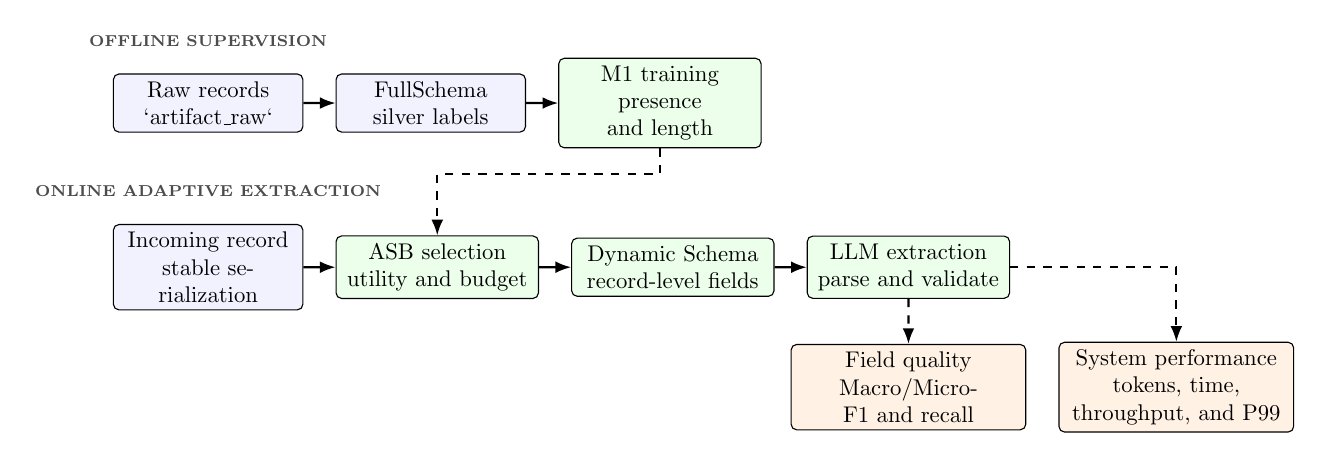
\begin{tikzpicture}[scale=0.82,transform shape,
  node distance=5mm and 5mm,
  data/.style={draw, rounded corners=2pt, align=center, minimum height=9mm,
    text width=27mm, fill=blue!5},
  process/.style={draw, rounded corners=2pt, align=center, minimum height=9mm,
    text width=29mm, fill=green!8},
  eval/.style={draw, rounded corners=2pt, align=center, minimum height=9mm,
    text width=34mm, fill=orange!10},
  stage/.style={font=\bfseries\scriptsize, text=black!70},
  arrow/.style={-{Latex[length=2mm]}, thick},
  dependency/.style={-{Latex[length=2mm]}, thick, dashed},
  evalarrow/.style={-{Latex[length=2mm]}, thick, dashed}
]
\node[stage] (offline-title) {OFFLINE SUPERVISION};
\node[data, below=3mm of offline-title] (raw) {Raw records\\`artifact\_raw`};
\node[data, right=of raw] (silver) {FullSchema\\silver labels};
\node[process, right=of silver] (train) {M1 training\\presence and length};
\draw[arrow] (raw) -- (silver);
\draw[arrow] (silver) -- (train);

\node[stage, below=7mm of raw] (online-title) {ONLINE ADAPTIVE EXTRACTION};
\node[data, below=3mm of online-title] (record) {Incoming record\\stable serialization};
\node[process, right=of record] (select) {ASB selection\\utility and budget};
\node[process, right=of select] (schema) {Dynamic Schema\\record-level fields};
\node[process, right=of schema] (llm) {LLM extraction\\parse and validate};
\draw[dependency] (train.south) -- ++(0,-4mm) -| (select.north);
\draw[arrow] (record) -- (select);
\draw[arrow] (select) -- (schema);
\draw[arrow] (schema) -- (llm);

\node[eval, below=7mm of llm] (quality) {Field quality\\Macro/Micro-F1 and recall};
\node[eval, right=of quality] (performance) {System performance\\tokens, time, throughput, and P99};
\draw[evalarrow] (llm.south) -- (quality.north);
\draw[evalarrow] (llm.east) -| (performance.north);
\end{tikzpicture}%
}
\caption{Overall study design. Raw records construct FullSchema silver-label supervision for M1
training. The online path applies ASB selection before dynamic-Schema extraction. Field-quality and
system-performance evaluations use distinct workloads; silver labels support method development and
presence evaluation, but do not constitute an independent human Gold reference.}
\label{fig:overall-framework}
\end{figure}

\section{数据与监督信号}

项目数据库中的原始记录表 \texttt{artifact\allowbreak\_raw} 与已有的完整抽取结果表
\texttt{artifact\allowbreak\_extract} 通过
记录标识字段 `artifact_id` 对齐。`artifact_id` 是一条文化遗产记录的唯一标识，仅用于
跨表连接、数据划分和跨批次结果配对，不作为模型输入特征。内连接得到 6,763 条记录；本实验的
候选字段集合 $F$ 包含 18 个预先定义的目标抽取字段，而非原始 JSON 中任意可见的键。数据划分为训练集
5,410 条、验证集 677 条和测试集 676 条。
`gold_main` 为测试集中的 500 条冻结子集，不与训练集或验证集重叠。

表~\ref{tab:field-schema}给出候选字段的语义角色、预设任务权重和训练集中的银标非空率。字段权重
是任务价值先验，`name` 与 `category` 为必选字段，始终保留；其余字段由选择器按记录决定。
FullSchema 包含 $F$ 的全部字段，动态 Schema 是记录 $r$ 的子集 $S_r\subseteq F$，字段选择的
最小单位是目标抽取字段，而非原始 JSON 键。

\begin{table}[htbp]
\centering
\footnotesize
\caption{Candidate extraction fields and their roles in the cultural-heritage Schema. Prevalence is the
non-empty rate of the FullSchema-derived silver reference in the 5,410-record training split. Weights are
pre-specified task values rather than estimates learned from this dataset.}
\label{tab:field-schema}
\resizebox{\linewidth}{!}{%
\begin{tabular}{@{}>{\raggedright\arraybackslash}p{.25\textwidth}>{\raggedright\arraybackslash}p{.24\textwidth}c c>{\raggedright\arraybackslash}p{.20\textwidth}@{}}
\toprule
Fields & Semantic role & Weight & Required & Training prevalence \\
\midrule
`name`, `category` & Object identity and category & 1.0, 0.9 & Yes & 100.0\%, 100.0\% \\
`form_type`, `material`, `period` & Form, material, and dating & 0.9, 0.9, 0.8 & No & 98.8\%, 99.7\%, 99.8\% \\
`dynasty`, `usage` & Historical attribution and function & 0.9, 0.7 & No & 74.8\%, 63.3\% \\
`motif`, `related_person`, `culture` & Decoration, related person, and cultural attribution & 0.7, 0.5, 0.6 & No & 23.9\%, 13.8\%, 6.9\% \\
`region`, `craft_school`, `acq_type` & Provenance region, production school, and acquisition & 0.6, 0.6, 0.4 & No & 3.5\%, 1.8\%, 1.6\% \\
`condition`, `site`, `related_event`, `craft` & Condition, site, related event, and technique & 0.6, 0.6, 0.4, 0.6 & No & 0.9\%, 0.8\%, 0.6\%, 0.5\% \\
`desc` & Narrative description & 0.5 & No & 100.0\% \\
\bottomrule
\end{tabular}
}
\end{table}

`artifact_extract` 不是人工真值。它是既有 FullSchema 过程产生的 model-assisted
silver reference。对字段 $f$，非空 FullSchema 输出构造 `present=1`，空值构造
`present=0`；非空字段值使用 `cl100k_base` 统计 Token 数作为长度标签。因此模型
学到的是 FullSchema 输出行为，而非已被独立人工确认的事实真实性。该边界同时适用于
第一部分离线评估和 `gold_main` 的字段存在性评价。

Presence Macro-F1 和 Micro-F1 分别衡量跨字段均衡表现与字段实例加权表现；Exact Value
Recall、Coverage 和 Total tokens 用于共同描述值级一致性、字段覆盖和调用负载。Length MAE
仅评价银标非空字段的长度预测，不能解释为真实 API Token 误差。

训练规模消融使用 50、100、250、500、1000、2500 和 5410 条，每个规模使用 5 个
seed。本文将 $n$ 定义为用于训练 M1 的 FullSchema 银标记录数；它不是测试记录数，
也不是单次 LLM 请求的字段数。seed 是控制训练初始化、数据顺序和抽样过程的随机种子，
用于检查结果是否依赖某一次随机运行。固定 seed 下采用多标签缺口贪心顺序构造嵌套训练
前缀，因此小规模样本是大规模样本的前缀，不应视为完全独立的均匀抽样。后文的“100 条
银标启动样本三种子主结果”特指稳定版 Prompt 下三个随机种子的真实 LLM 对照，不与本节
表格中的五个随机种子离线模型消融混用。

\section{方法实现}

\subsection{基于稀疏文本特征的字段预测器}

\subsubsection{输入、标签与监督目标}

对每条原始记录 $r$，系统将其 JSON 键值及描述文本稳定序列化为
\texttt{record\allowbreak\_text}；同一条
记录的字符级与词级特征向量由该文本共同构成，并供所有候选字段共享使用。字段 $f$ 的
存在性标签定义为 $y_f(r)\in\{0,1\}$：FullSchema 银标中该字段非空时为 1，空值时为 0。
仅当 $y_f(r)=1$ 时，才以该字段值经 `cl100k_base` 编码得到的 Token 数 $o_f(r)$ 作为长度
监督。训练、验证和测试记录按 `artifact_id` 划分且互不重叠；验证集只用于字段阈值校准，
测试集不参与任一训练或校准步骤。因而 M1 预测的是完整 Schema 抽取的银标行为，
而不是经人工独立确认的字段事实。

\subsubsection{共同训练协议与训练规模设计}

三种模型均对 18 个候选字段逐字段训练存在性分类器，而不是训练一个共享的多标签输出层；
每个分类器均采用 `class_weight=balanced`、`liblinear` 求解器、最多 1,000 次迭代，并以当前
随机种子初始化。所有 TF--IDF 词表和 IDF 权重仅在对应训练子集拟合，再变换验证集和测试集，
以避免信息泄漏。长度预测在正样本不足时回退为中位数，否则拟合
$\log(1+o_f(r))$；分类和长度分支共享相同的标签与划分。

训练规模实验使用 $n\in\{50,100,250,500,1000,2500,5410\}$，并在五个固定随机种子
（42--46）下重复。每个较小规模训练集是同一 seed 对应较大规模训练集的嵌套前缀；前缀由
多标签缺口贪心排序构造，以尽可能维持各字段的正例比例。这一设计使规模曲线比较的是监督量，
而非彼此无关的抽样波动。Character、M1 和 M2 均在全部训练规模上测量，因此图~\ref{fig:offline-main}
可直接比较三种特征融合策略的规模趋势。M2 仅用于离线消融，不进入在线实验。

\subsubsection{Character TF--IDF 基线}

字符级基线仅使用字符级 TF--IDF 表示
\texttt{record\allowbreak\_text}，不依赖中文分词；它是后续融合模型的
共同参照，而非在线字段选择器。其长度分支遵循共同训练协议。

\subsubsection{M1：早融合字段预测器}

M1 将字符级和词级 TF--IDF 表示拼接为稀疏矩阵，对每个字段独立输出存在性分数
$p(r,f)$ 和长度估计 $\hat{o}(r,f)$。字段阈值在验证集校准后用于测试集，长度预测采用
对数变换、逆变换和非负截断。

训练集中始终非空的 `name`、`category` 和 `desc` 使用常量预测；这些字段的高 F1 不代表
模型学到了可迁移的区分能力。相反，`craft`、`site`、`acq_type`、`craft_school` 和
`related_event` 等长尾字段的正样本不足，是 M1 宏平均表现的主要限制。存在性概率与长度
估计分别刻画了“该字段可能有值”和“该字段可能带来的输出负载”，二者不应被解释为字段值
正确性或真实 API Token 的直接预测。

\subsubsection{M2：后融合消融模型}

M2 使用与 M1 相同的两类 TF--IDF 特征，但分别训练字符模型和词模型，再在验证集融合其
存在性概率：
\begin{equation}
p_{\mathrm{M2}}(r,f)=\alpha p_{\mathrm{char}}(r,f)+(1-\alpha)p_{\mathrm{word}}(r,f).
\end{equation}
其长度分支与 M1 一致。因此，M2 只检验存在性概率的融合位置，仅用于离线消融。

\subsubsection{与预算选择器的接口及边界}

M1 在 LLM 调用前运行，不生成字段值。其输出 $p(r,f)$ 与 $\hat{o}(r,f)$ 输入效用和成本
函数，再由必选字段约束与 0--1 背包选择器产生 $S_r$。TF--IDF 与线性模型提供低延迟、
可检查的裁剪信号；预算仅限制调用前的估计字段组合，实际 Token 由在线实验测量。

\begin{center}
\centering
\resizebox{\linewidth}{!}{%
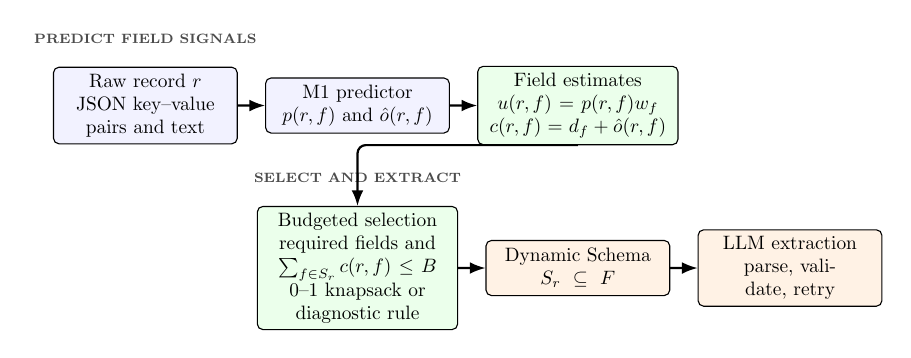
\begin{tikzpicture}[scale=0.70,transform shape,
  node distance=5mm and 5mm,
  input/.style={draw, rounded corners=2pt, align=center, minimum height=10mm,
    text width=31mm, fill=blue!5},
  decision/.style={draw, rounded corners=2pt, align=center, minimum height=10mm,
    text width=34mm, fill=green!8},
  output/.style={draw, rounded corners=2pt, align=center, minimum height=10mm,
    text width=31mm, fill=orange!10},
  arrow/.style={-{Latex[length=2mm]}, thick},
  stage/.style={font=\bfseries\scriptsize, text=black!70}
]
\node[stage] (predict-title) {PREDICT FIELD SIGNALS};
\node[input, below=3mm of predict-title] (record) {Raw record $r$\\JSON key--value pairs and text};
\node[input, right=of record] (m1) {M1 predictor\\$p(r,f)$ and $\hat{o}(r,f)$};
\node[decision, right=of m1] (score) {Field estimates\\$u(r,f)=p(r,f)w_f$\\$c(r,f)=d_f+\hat{o}(r,f)$};
\draw[arrow] (record) -- (m1);
\draw[arrow] (m1) -- (score);
\node[stage, below=6mm of m1] (select-title) {SELECT AND EXTRACT};
\node[decision, below=3mm of select-title] (select) {Budgeted selection\\required fields and $\sum_{f\in S_r}c(r,f)\leq B$\\0--1 knapsack or diagnostic rule};
\node[output, right=of select] (schema) {Dynamic Schema\\$S_r\subseteq F$};
\node[output, right=of schema] (llm) {LLM extraction\\parse, validate, retry};
\draw[arrow, rounded corners=3pt] (score.south) -| (select.north);
\draw[arrow] (select) -- (schema);
\draw[arrow] (schema) -- (llm);
\end{tikzpicture}
}
\captionof{figure}{ASB dynamic-Schema decision architecture. M1 predicts field presence and output length
from each raw record; the selector combines field value, estimated cost, and required-field constraints
to construct a record-level Schema. The SchemaRAG comparator bypasses M1 and budgeted cost, using an
independent query--field embedding Top-$k$ ranking.}
\label{fig:asb-decision}
\end{center}

\subsection{实验策略定义}

为避免把不同性质的对照混在一起，本文将策略分为完整 Schema 基线、仅依赖提示词的
基线、固定字段诊断、本方法的动态策略和外部方法五类。各策略的字段选择规则如下。

\begin{center}
\centering
\scriptsize
\renewcommand{\arraystretch}{0.88}
\captionof{table}{Inputs, selection mechanisms, and comparison roles of extraction strategies.}
\label{tab:strategies}
\resizebox{\linewidth}{!}{%
\begin{tabular}{>{\raggedright\arraybackslash}p{2.2cm}>{\raggedright\arraybackslash}p{3.3cm}>{\raggedright\arraybackslash}p{5.5cm}>{\raggedright\arraybackslash}p{3.4cm}}
\toprule
Strategy & Input fields & Field-selection or prompt mechanism & Comparison role\\
\midrule
`full` & All 18 fields & No pruning; base extraction prompt & Full-Schema baseline\\
`prompt-null` & All 18 fields & Output `null` without reliable evidence & Strict prompt-only baseline\\
`prompt-omit` & All 18 fields & Permit omitted fields without reliable evidence & Prompt-only output control\\
`fixed-5/10` & Fixed 5 or 10 fields & Fixed field weights; ignores the current record & Fixed-field diagnostic\\
`budget-200/400` & Record-level field subset & M1 prediction followed by a capacity-specific 0--1 knapsack & Dynamic strategy\\
`lambda` & Record-level field subset & M1 prediction followed by a net-utility threshold & No-hard-budget control\\
`SchemaRAG k=10/15` & Top-$k$ field subset & Cosine ranking of query and field vectors & External reimplementation\\
\bottomrule
\end{tabular}
}
\end{center}

`full` 始终向 LLM 提供本实验的 18 个候选字段，不使用 M1，是输入完整性和在线负载的
主要基线。`prompt-null` 与 `prompt-omit` 也保留完整 Schema，只改变指令：前者要求
无可靠依据时输出 `null`，后者允许省略字段。因此它们可以检验仅依靠 Prompt 是否
能够替代实际的 Schema 裁剪，但不能减少 Schema 输入负载。`fixed-5` 和 `fixed-10`
不读取当前记录内容，而是按预先固定的字段权重取字段；由于其字段集合主要包含数据
中较稠密的字段，存在先验偏置，只作为补充诊断，不参与动态方法的公平主排序。

`budget-200` 和 `budget-400` 由 M1 预测字段存在性和长度，再以字段效用及估计成本为输入，
在强制保留必选字段的条件下用 0--1 背包分别求解容量为 200 和 400 的子集。无硬预算对照
按净收益 $u(r,f)-\lambda c(r,f)$ 选字段，取 $\lambda=0.003$；该值是当前效用--成本标度下的
实验门槛，不是 API 价格、Token 上限或跨数据集的最优值。

估计字段成本仅用于调用前决策：
\begin{equation}
 \widehat{C}_{field}(r,f)=C_{schema}(f)+\widehat{C}_{output}(r,f).
\end{equation}
它不是实际 API 成本；实际 `input_tokens`、`output_tokens` 和 `total_tokens` 在调用后由
API usage 记录，并累计重试开销。原始记录输入通常无论选择多少字段都要发送，因此不计入
字段组合预算，但计入在线 Token 统计。

\subsection{基于 Embedding 的 SchemaRAG 外部适配实现}

SchemaRAG 在本文中作为独立的语义检索式字段选择器实现，不使用 M1 预测或预算背包；它以
记录--字段描述的语义相似度替代记录级标签学习，所选字段进入相同的下游 LLM 抽取流程。

\subsubsection{检索表示与字段排序}

对每个字段 $f$，实现分别对字段名和字段定义调用 Embedding 服务，以 0.5/0.5 加权后
进行 L2 归一化，得到字段向量 $\bar{e}(f)$。对记录 $r$，将固定检索指令与稳定序列化的
原始记录拼接为 query 文本，并用同一服务得到归一化 query 向量 $\bar{e}(r)$。字段按
余弦相似度排序：
\begin{equation}
 s(r,f)=\left\langle\bar{e}(r),\bar{e}(f)\right\rangle,
 \qquad S_r=\operatorname{TopK}_{f\in F}s(r,f).
\end{equation}
由于向量已归一化，上式的点积等价于余弦相似度。实现从 18 个候选字段中选择 Top-10
或 Top-15 字段，并以 $S_r$ 构造记录级动态 Schema：

\begin{center}
\texttt{raw record -> query embedding -> cosine ranking -> Top-k fields -> LLM}
\end{center}

\subsubsection{在线开销与统一结果接口}

字段向量按配置哈希缓存；每条记录的 query embedding 在线生成并计入端到端时间，分别记录
`schema_embedding_ms` 和 `query_embedding_ms`。统一结果接口中的估计成本不参与 Top-k 排序，
实测 Token 和在线时间仍以 LLM 调用及检索请求记录为准。

\subsubsection{适配范围与复现边界}

该方法依据公开描述完成，是固定 Top-k 字段检索的外部适配实现，不包含字段分段、示例检索
或二阶段重排序；因此，比较仅限于当前实现、模型服务和实验条件，不代表官方复现或完整
SchemaRAG 系统的性能上限。

\subsection{在线执行与指标实现}

当前实现是单进程异步有界 Producer--Consumer。并发参数 `c` 控制 Consumer 数量，
队列容量 `q` 控制 `asyncio.Queue` 大小；队列满时 Producer 阻塞形成背压。任务按照
输入顺序增量构造，成功任务按方法和配置哈希断点续跑，失败任务在最多两次重试后
保留错误状态。

\begin{equation}
 \mathrm{makespan}=t_{finish}-t_{start},\qquad
 \mathrm{effective\ throughput}=\frac{N_{success}}{\mathrm{makespan}}.
\end{equation}

`pipeline_ms` 的起止点覆盖在线记录读取、任务构造、入队、LLM 请求、重试和结果写入。
它不包含 100 条 FullSchema 启动样本生成、训练数据和银标标签构造、M1 离线训练、
模型或向量器加载。当前 M1 使用既有 `training_dataset.jsonl`，训练本身不调用 LLM。
因此本文系统结果是在线推理结果，不是全生命周期成本结果。选择 `budget-200` 也不是
因为它对应某个 API 的 200-token 限额，而是因为离线回放中它在容量、字段覆盖和请求
负载之间提供了中间 operating point；真实 LLM 三 seed 中它相较 `budget-400` 和
无硬容量的 lambda 对照具有更低 Token，同时字段指标没有出现明显崩溃。这个选择是
当前数据和服务条件下的工程折中，不应写成全局最优预算。

为明确在线执行边界，图~\ref{fig:online-execution} 展示单进程 Runner 的数据流。Producer
只负责读取、规划和入队；Consumer 负责请求、解析、校验和有限重试；Writer 负责持久化
结果与运行指标。有界队列是背压位置，不表示已经实现多进程或跨节点调度。

\begin{figure}[htbp]
\centering
\resizebox{\linewidth}{!}{%
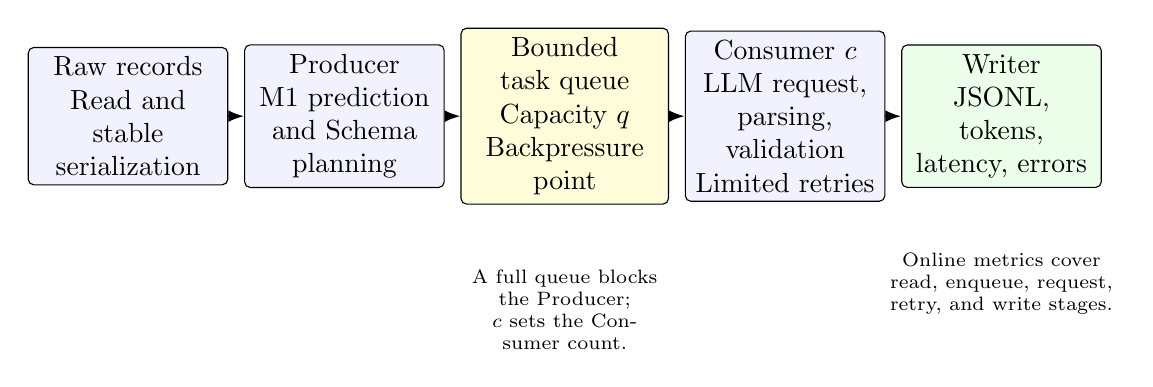
\begin{tikzpicture}[
  node distance=4mm and 2mm,
  block/.style={draw, rounded corners=2pt, align=center, minimum height=9mm,
    text width=23mm, fill=blue!5},
  queue/.style={draw, rounded corners=2pt, align=center, minimum height=12mm,
    text width=24mm, fill=yellow!15},
  output/.style={draw, rounded corners=2pt, align=center, minimum height=9mm,
    text width=23mm, fill=green!8},
  arrow/.style={-{Latex[length=2mm]}, thick},
  note/.style={font=\scriptsize, align=center, text width=29mm}
]
\node[block] (source) {Raw records\\Read and stable serialization};
\node[block, right=of source] (producer) {Producer\\M1 prediction and Schema planning};
\node[queue, right=of producer] (queue) {Bounded task queue\\Capacity $q$\\Backpressure point};
\node[block, right=of queue] (consumer) {Consumer $c$\\LLM request, parsing, validation\\Limited retries};
\node[output, right=of consumer] (writer) {Writer\\JSONL, tokens, latency, errors};
\draw[arrow] (source) -- (producer);
\draw[arrow] (producer) -- (queue);
\draw[arrow] (queue) -- (consumer);
\draw[arrow] (consumer) -- (writer);
\node[note, below=7mm of queue] {A full queue blocks the Producer;\\$c$ sets the Consumer count.};
\node[note, below=7mm of writer] {Online metrics cover read, enqueue, request,\\retry, and write stages.};
\end{tikzpicture}
}
\caption{Online execution architecture. A single-process asynchronous Runner connects the Producer,
Consumer, and Writer through a bounded queue; model loading, M1 training, and startup-sample generation
are one-time costs outside the pipeline.}
\label{fig:online-execution}
\end{figure}

\section{第一部分：离线选择能力}

\subsection{训练规模与模型策略消融}

表~\ref{tab:offline} 比较字符级 TF--IDF 基线、M1 早融合模型与 M2 后融合消融模型，均使用
100 条银标记录训练并在五个随机种子上取平均。三者共享相同的字段标签、训练/验证/测试划分
和条件式长度回归，因此该对照只检验输入表征及存在性概率的融合位置。字符级基线的
Macro-F1 为 0.5187，高于 M1 的 0.5088 和 M2 的 0.5083；相反，M1 的 Micro-F1 为 0.9343，
高于基线的 0.9126，M2 为 0.9341。M1 的 Length MAE 为 4.7615，略低于基线的 4.8046。
因此，早融合在当前设置下改善的是总体实例加权表现和长度估计，而未改善对长尾字段更敏感的
Macro-F1；这些离线差异不能解释为长尾字段的普遍改进，在线主实验仅采用 M1。 

\begin{table}[htbp]
\centering
\caption{Offline ablation of model strategies trained on 100 silver-label records (mean over five seeds).}
\label{tab:offline}
\begin{tabular}{lccc}
\toprule
Model & Presence Macro-F1 & Presence Micro-F1 & Length MAE\\
\midrule
Character TF--IDF & 0.5187 & 0.9126 & 4.8046\\
M1: character + word TF--IDF & 0.5088 & 0.9343 & 4.7615\\
M2: probability fusion & 0.5083 & 0.9341 & 4.7615\\
\bottomrule
\end{tabular}
\end{table}

图~\ref{fig:offline-main}在 50--5410 条样本和五个随机种子下比较三种模型的规模趋势；
M2 的长度分支与 M1 共享特征，因此不将其解释为独立的长度建模优势。

\begin{center}
\centering
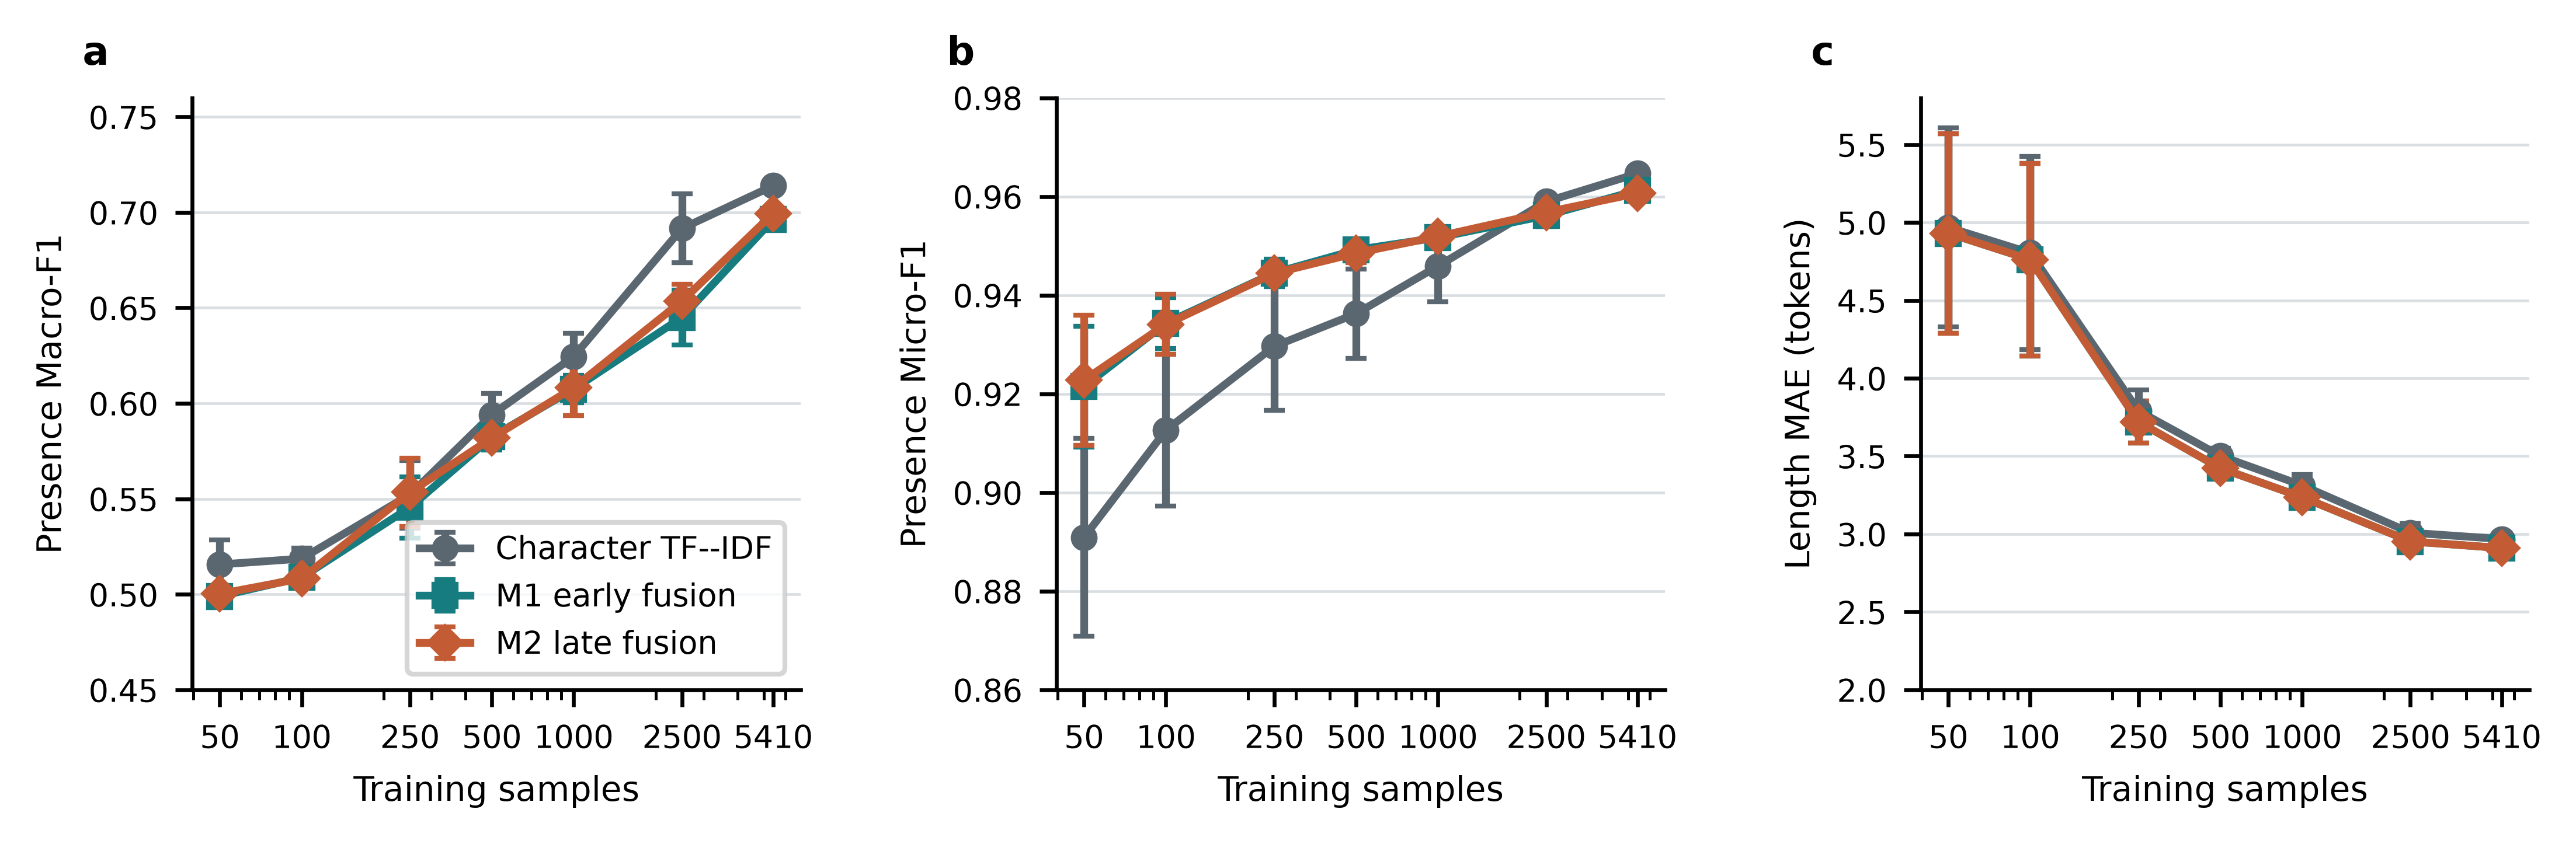
\includegraphics[width=\linewidth]{model_strategy_learning_curves.png}
      \captionof{figure}{Offline learning curves for Character TF--IDF, M1 early fusion, and M2 late fusion
 across all training-set sizes. Points and error bars show means and 95\% confidence intervals across five
 random seeds. Character TF--IDF retains higher Macro-F1 at large training sizes, whereas M1 and M2 show
 similar Micro-F1 and length trends. These measures assess FullSchema-derived silver-label selection
 behaviour, not factual extraction accuracy or actual API-token cost.}
\label{fig:offline-main}
\end{center}

随着训练规模增加，M1 和 M2 的 Micro-F1 与 Length MAE 均改善，但两种融合策略没有显示出
稳定的相互优势；在完整训练规模下，字符级基线的 Macro-F1 仍更高。因此，后融合未在当前
配置下提供明确整体收益，在线实验采用 M1。Length MAE 评价的是银标长度标签，不是实测 Token。

图~\ref{fig:offline-budget}考察不同训练规模下 M1 对完整训练选择行为的恢复程度；
Coverage 和 Recovery 均是离线选择指标，不代表字段值的事实正确性。

\begin{center}
\centering
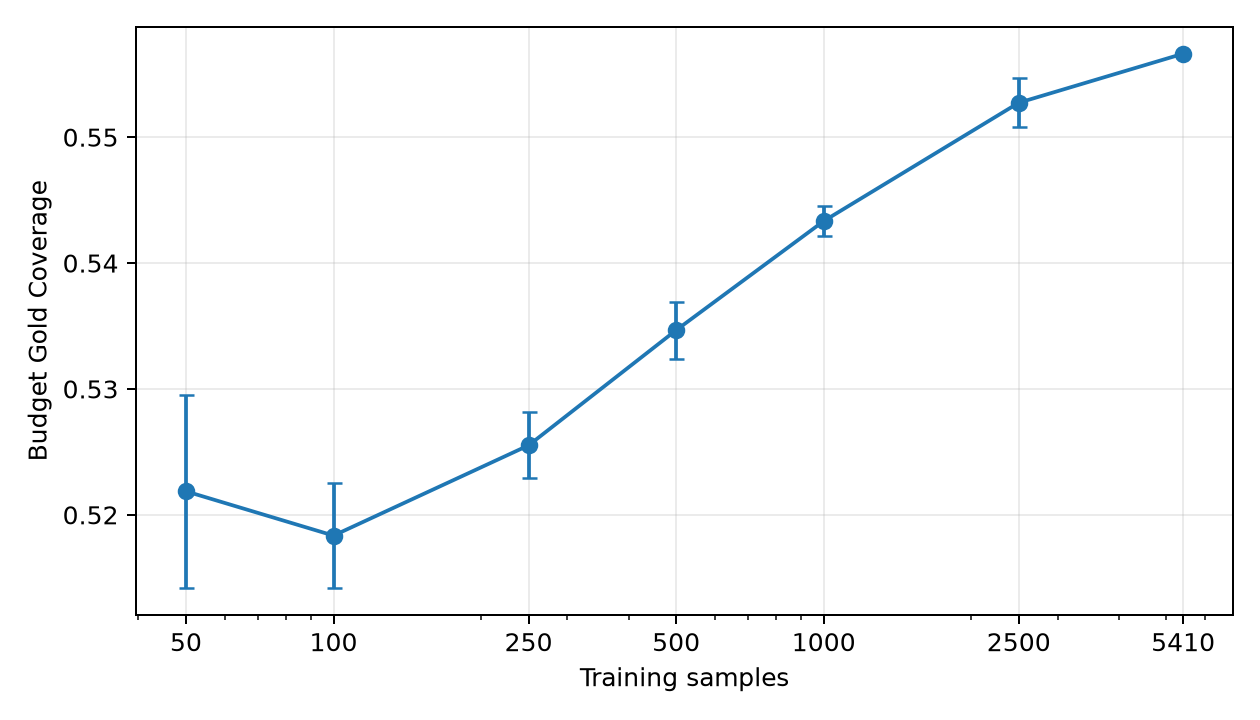
\includegraphics[width=.47\linewidth]{budget_coverage.png}\hfill
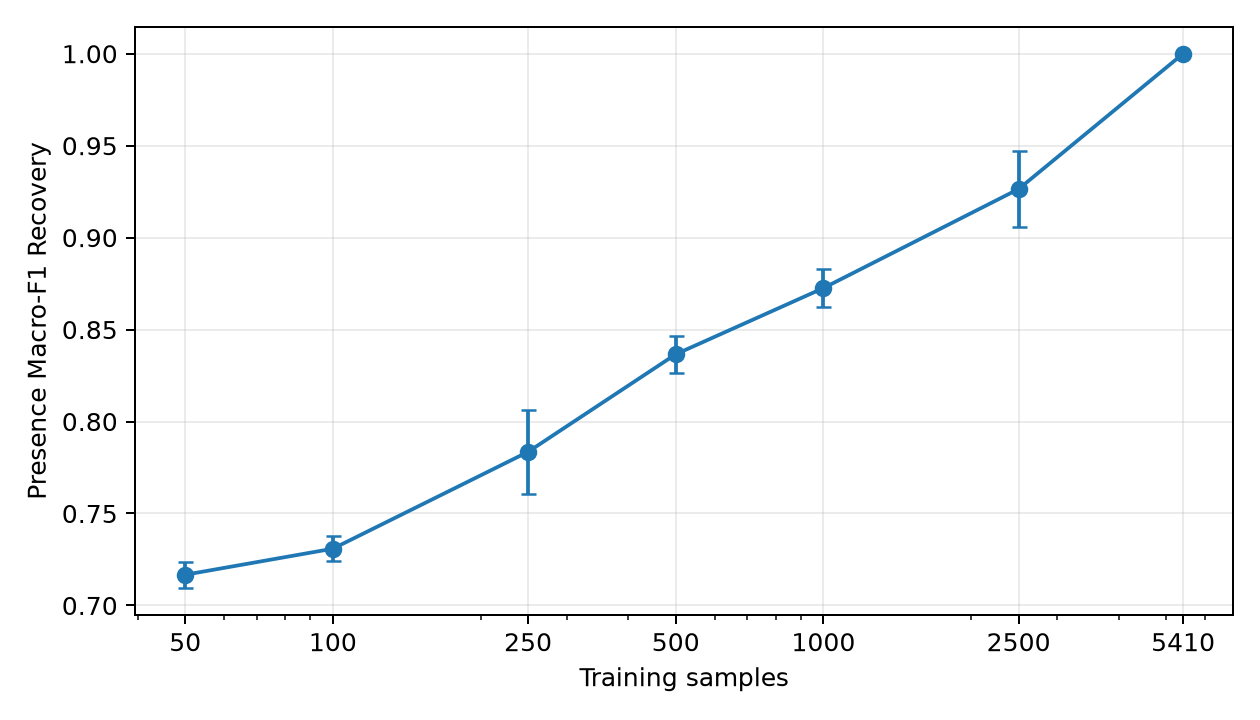
\includegraphics[width=.47\linewidth]{recovery.png}
\captionof{figure}{Budget coverage and recovery relative to the full model across M1 training-set sizes. Coverage
denotes selected-field coverage of nonempty FullSchema fields, not factual value accuracy; recovery
contextualizes the engineering compromise at $n=100$.}
\label{fig:offline-budget}
\end{center}

图~\ref{fig:offline-budget}表明，小样本首先恢复高频字段的选择行为；因此 $n=100$ 代表
低监督下的可用工程折中，而非所有字段均接近完整训练。

\subsection{离线预算回放}

在 6,763 条记录上，预算 100、200 和 400 的平均估计字段成本分别为 90.52、192.67 和
385.04，平均选中字段数为 2.75、4.81 和 8.23，FullSchema 非空字段覆盖率为
26.06\%、53.46\% 和 94.95\%。预算增大确实提高了离线覆盖，但该覆盖率不能替代
重新调用 LLM 后的值质量，也不能直接当作 API 账单。

\section{第二部分：冻结测试集上的 LLM 抽取结果}

离线实验表明，预算约束改变了字段覆盖，但选中字段不等于值被正确抽取。本节在 500 条
冻结记录上比较字段质量、值级一致性、Coverage 和 Token，随后验证三个随机种子的重复性，
并与 FullSchema 和 SchemaRAG 进行边界对照。所有字段指标均相对于模型辅助银标参照，在线
时间和吞吐量留待独立性能负载评价。

\subsection{多种 Schema 策略的内部对照}

正式实验在 500 条冻结评估记录上比较八种方法；所有内部方法使用匹配的模型服务和
调用条件。八种方法的共同成功配对集合为 476 条，因而表~\ref{tab:eight} 的比较重点
是同一批记录上的相对变化，而不是把失败记录差异误归因于字段选择策略。八种方法按
其在实验中的作用分为四组：`full` 提供完整 Schema 的高负载参照；`prompt-null` 和
`prompt-omit` 是仅依赖提示词的基线，用于检验提示词约束本身的作用；`fixed-5` 和
`fixed-10` 使用固定字段先验，仅用于诊断当前数据中高密度字段的上限；`budget-200`、
`budget-400` 和 `lambda=0.003` 则使用 M1 的记录级预测结果进行字段选择，分别考察
硬容量和软成本惩罚下的质量--Token 权衡。表中同时报告字段指标、覆盖率和总 Token，
以避免用单一质量或负载指标决定主方案。

\begin{table}[htbp]
\centering
\scriptsize
\caption{Comparison of eight internal methods on 476 jointly successful records.}
\label{tab:eight}
\resizebox{\linewidth}{!}{%
\begin{tabular}{lccccc}
\toprule
Method & Macro-F1 & Micro-F1 & Exact Recall & Coverage & Total tokens\\
\midrule
full & .7623 & .7410 & .6528 & 1.0000 & 539.83\\
prompt-null & .6215 & .5871 & .6557 & 1.0000 & 548.01\\
prompt-omit & .7475 & .7386 & .6078 & 1.0000 & 487.10\\
fixed-5 (diagnostic) & .8400 & .8382 & .6056 & .7725 & 344.74\\
fixed-10 (diagnostic) & .6633 & .6619 & .6353 & .8409 & 409.39\\
budget-200 & .7759 & .7780 & .6213 & .8303 & 381.49\\
budget-400 & .7736 & .7638 & .6606 & .9763 & 486.32\\
lambda=0.003 & .7822 & .7816 & .6407 & .9606 & 441.28\\
\bottomrule
\end{tabular}
}
\end{table}

表~\ref{tab:eight} 显示，完整字段集合不是质量上限：`prompt-null` 在相同完整 Schema
下的 F1 更低，提示词约束不能消除额外字段带来的假阳性。提高预算也不保证质量提升；
`budget-400` 的 Coverage 高于 `budget-200`，但 F1 未提高且总 Token 从 381.49 增至
486.32。`fixed-5` 的较高 F1 反映当前数据中的高密度字段先验，不能外推到字段组成不同
的记录。因此后续采用 `budget-200` 作为质量、覆盖和负载之间的工程折中，而非全局最优。

\subsection{主配置的跨随机种子验证}

在稳定版 Prompt 下，使用 100 条银标启动样本训练的三种 M1 策略均在每个随机种子上
完成全部 500 条记录。这里保持测试记录、LLM 服务、Prompt、字段评价协议和选择规则
不变，仅改变启动样本的随机种子及相应的模型拟合随机性，因此该实验回答的是有限监督
条件下的重复性问题，而不是跨数据分布的泛化问题。`budget-200` 的平均 Macro-F1、
Micro-F1、Exact Value Recall、Coverage 和总 Token 分别为 0.7644、0.7673、0.6470、
0.8381 和 385.5。

三种子下，`budget-200` 均完成 500 条冻结记录，平均 Macro-F1、Micro-F1、Exact Value
Recall、Coverage 和总 Token 分别为 0.7644、0.7673、0.6470、0.8381 和 385.5；
`lambda=0.003` 与 `budget-400` 分别将总 Token 增至 462.2 和 493.2，但未提高 F1。
这支持当前有限监督条件下的重复可用性，却不构成跨数据分布或模型服务的最优性证据。

\subsection{与完整 Schema 及外部检索策略的边界比较}

与历史完整 Schema 的比较首先提供负载层面的边界证据。新 M1 与历史 FullSchema 并非
同一调用批次；对共同的 476 个 `artifact_id` 进行对齐后，FullSchema 的平均总 Token
为 539.8，M1 `budget-200` 为 385.9，降低约 28.5\%。后者的 Micro-F1 数值更高，但
Exact Value Recall 略低，说明 Token 减少与不同质量指标的变化并不完全同向。这一结果
支持当前配置具有较低 Token 的工程观察，但由于调用批次不同，不能构成严格的显著性
检验，也不能排除批次、服务状态或其他未控制因素的影响。

SchemaRAG k=10/15 的 Macro-F1、Micro-F1 和总 Token 分别为 0.7069/0.7324、
0.7022/0.7224 和 432.9/503.6。M1 均值在当前实现和条件下呈现更高字段指标与较低
Token，但结果受 embedding 模型、Top-$k$、缓存和检索开销影响；该对照是公开描述基础上的
外部适配，不应外推为对官方方法或检索式 Schema 选择的整体否定。

因此，在当前字段集合、模型服务、Prompt 和模型辅助银标评价下，动态 Schema 可在较低
Token 下保持有竞争力的字段一致性，但不等同于人工事实准确率或跨任务最优性；端到端收益
需由独立性能负载另行检验。

\section{第三部分：在线预处理流水线}

\subsection{独立性能负载与实验条件}

性能负载为 2,000 条记录，来自训练集和验证集，不与第二部分测试集重叠。样本按原始
记录字节长度分为五个等频层，每层随机抽取 400 条，随机种子为 20260904。主实验比较
`full`、M1 `budget-200` 和 SchemaRAG k=10，使用 16 个并发消费者和容量为 16 的有界队列，
各重复三次。

\begin{table}[htbp]
\centering
\scriptsize
\setlength{\tabcolsep}{2pt}
\caption{Online-system results on the independent 2,000-record performance workload.}
\label{tab:system}
\begin{tabular}{@{}lccccc@{}}
\toprule
Method & Success rate & Makespan (s) & Effective throughput & Total tokens & P99 (ms)\\
\midrule
full & 100.0\% & 220.82 & 9.06 & 1,709,102 & 3,601\\
budget-200 & 100.0\% & 113.64 & 17.61 & 1,069,254 & 1,308\\
SchemaRAG k=10 & 99.9\% & 399.68 & 5.03 & 1,230,411 & 19,886\\
\bottomrule
\end{tabular}
\end{table}

图~\ref{fig:system-main}比较独立 2,000 条负载上的有效吞吐、总 Token、流水线时间和
尾延迟；结论仅限当前模型服务和并发配置。

\begin{figure}[htbp]
\centering
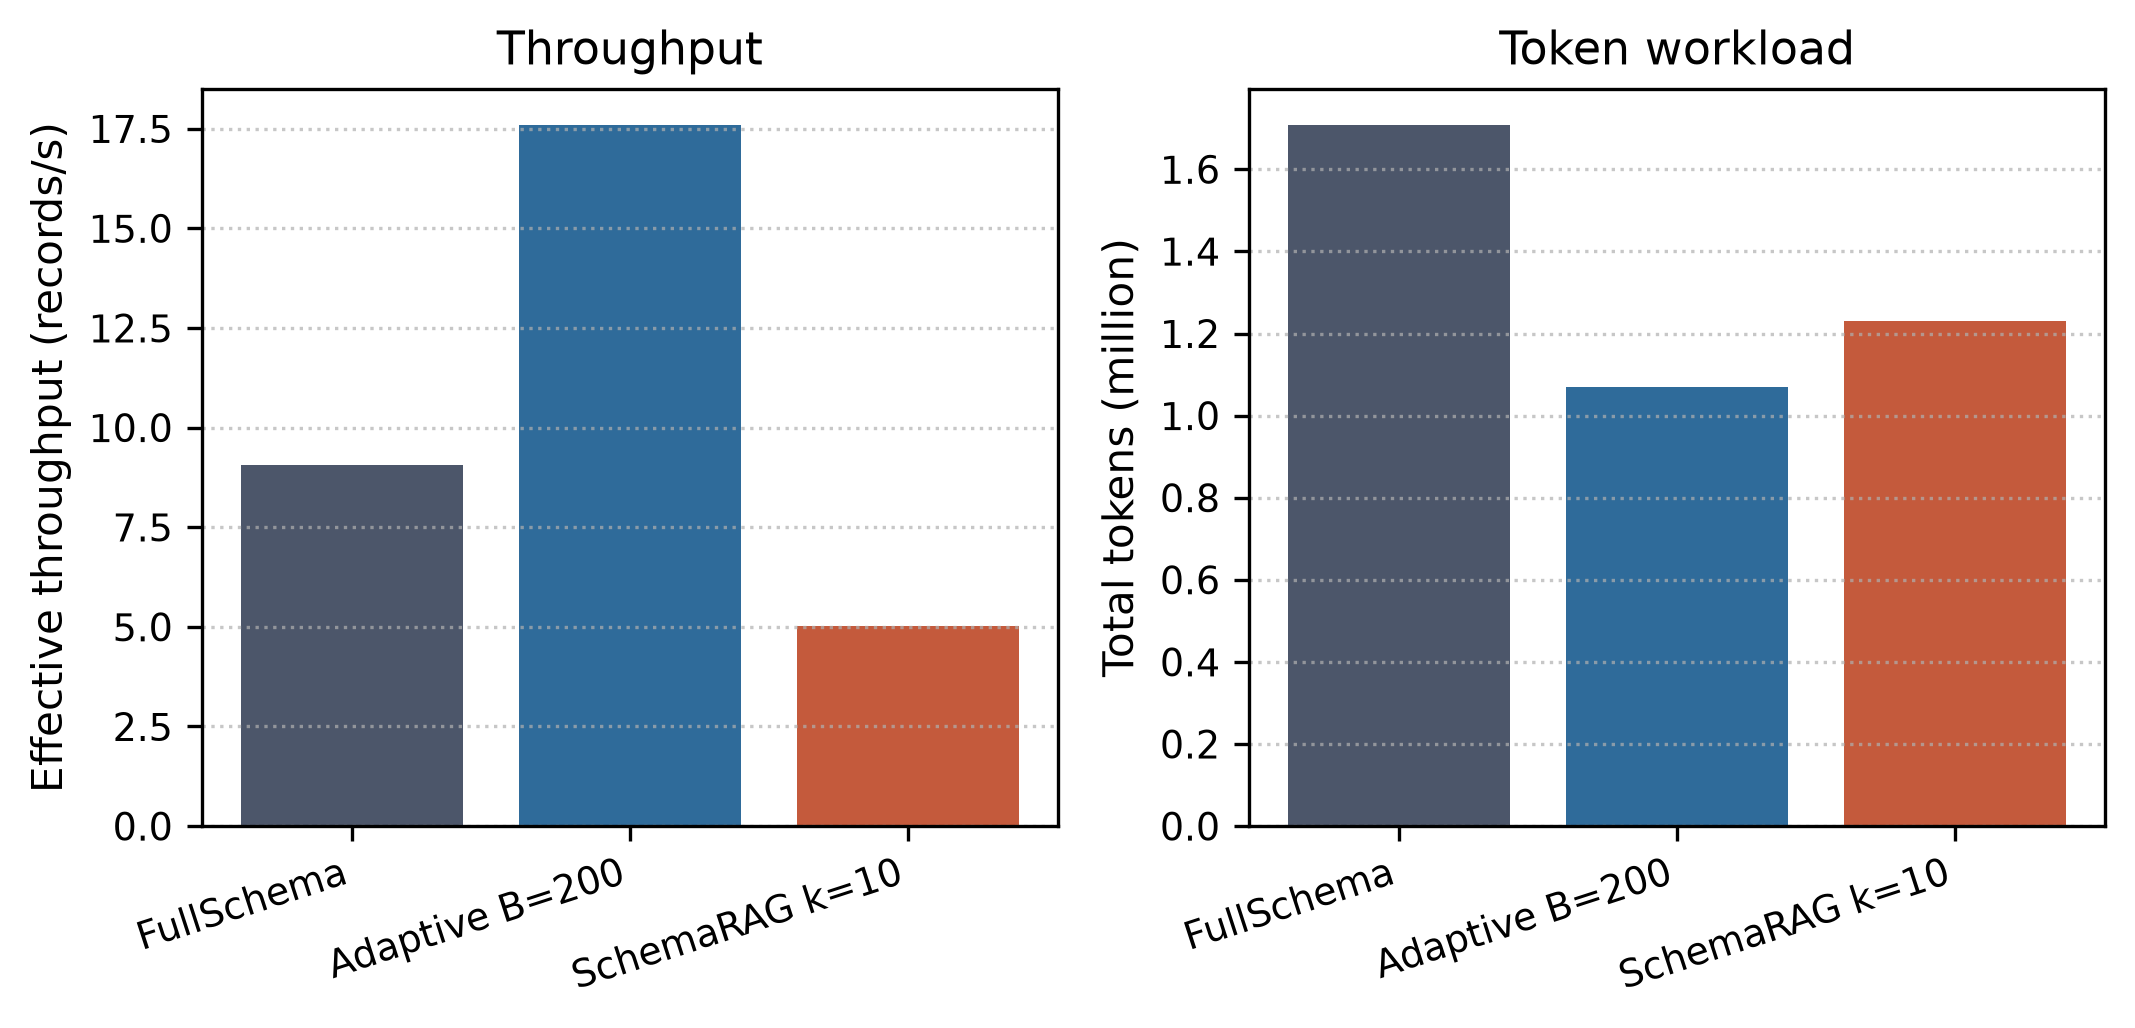
\includegraphics[width=.47\linewidth]{main_throughput_and_tokens.png}\hfill
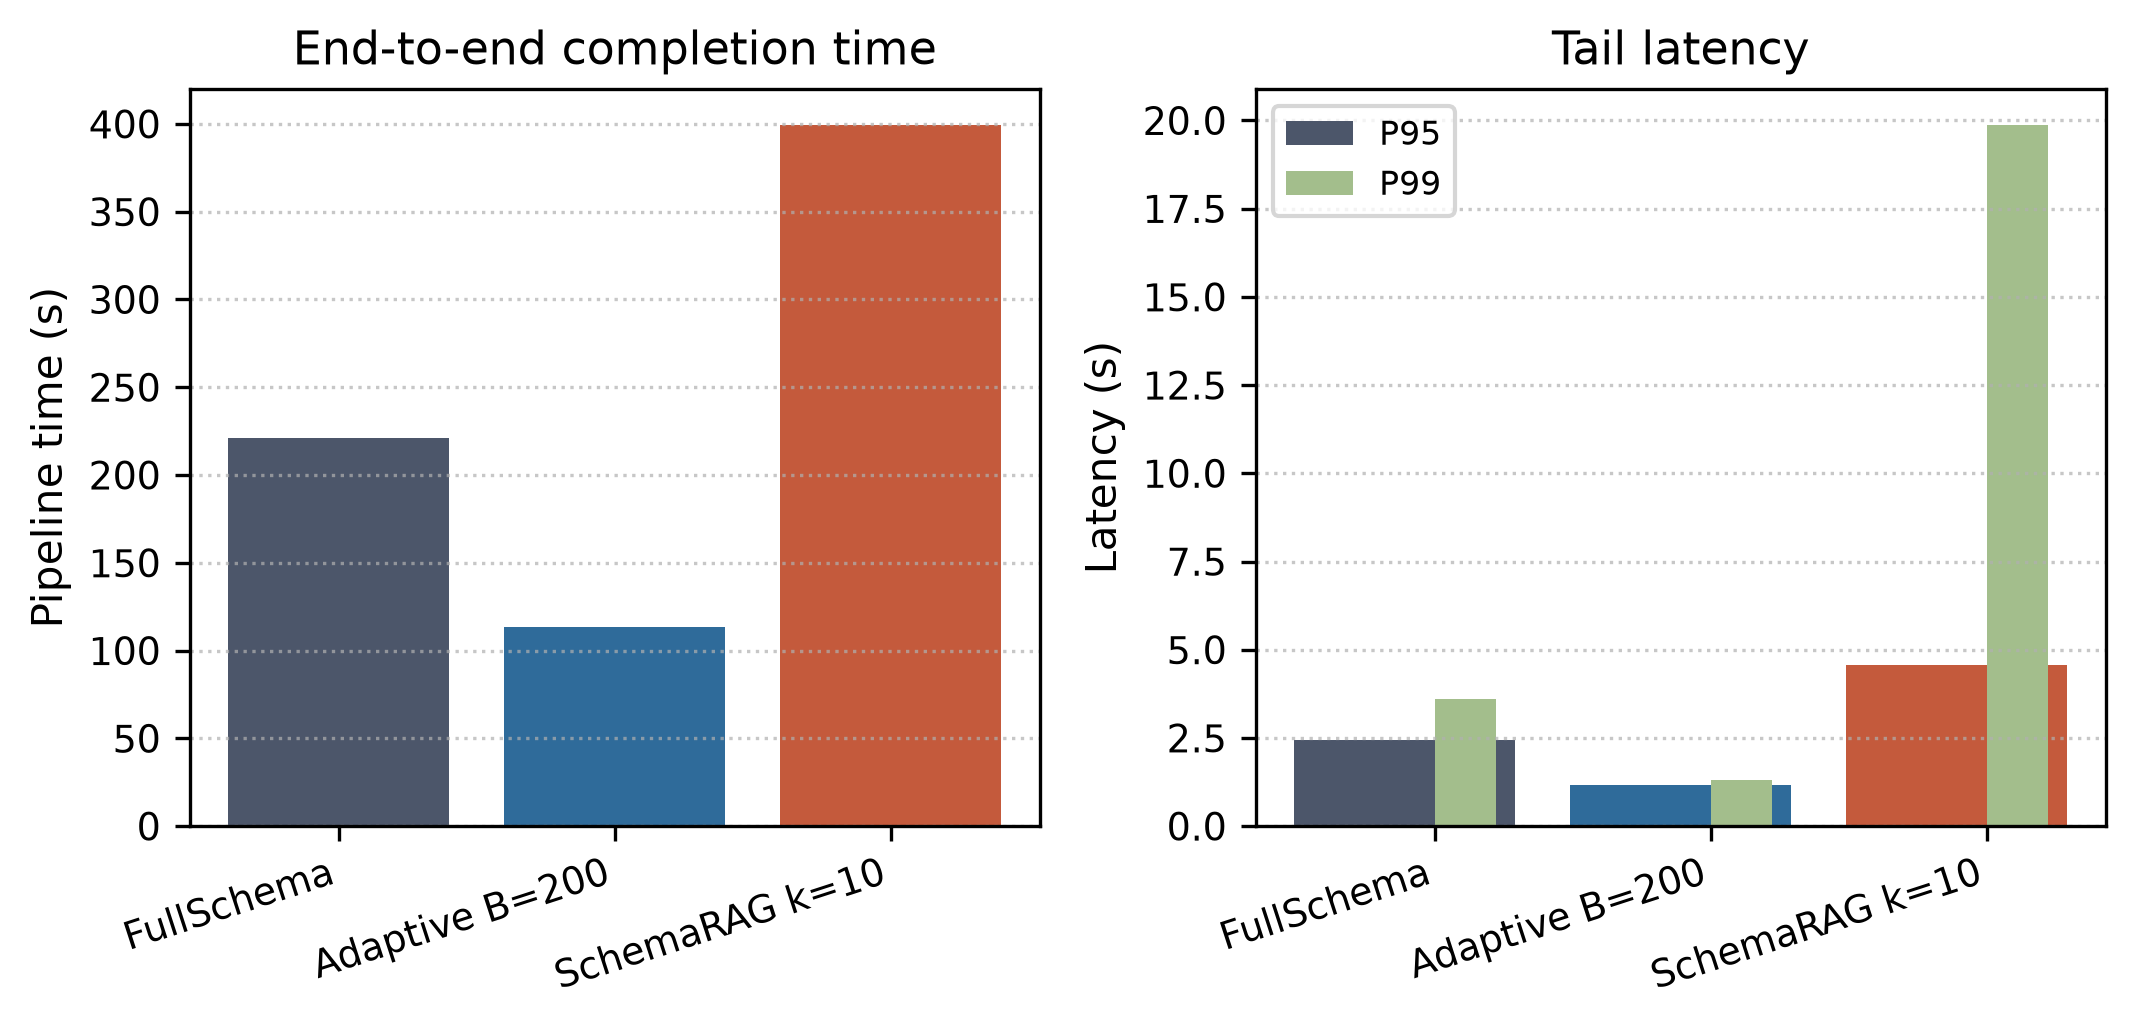
\includegraphics[width=.47\linewidth]{main_time_and_tail_latency.png}
\caption{Effective throughput, token workload, pipeline time, and tail latency in the main performance
experiment. The figure tests whether workload reduction transfers to system-level gains; it does not imply
universal scaling across service configurations.}
\label{fig:system-main}
\end{figure}

相对于 `full`，`budget-200` 的流水线时间降低 48.54\%、有效吞吐提高 94.38\%、总 Token
降低 37.44\%。SchemaRAG 虽少 28.01\% Token，却因累计约 258.61 s 的 query embedding
使整体时间增加 80.99\%、吞吐降低 44.43\%。因此字段负载收益必须以端到端计时验证。

\subsection{端点方向性验证}

为观察低并发和高并发端点，另在 500 条记录上比较 $c=1,q=1$ 与 $c=32,q=32$，
每种方法和端点重复两次。两种端点同时改变并发度和队列容量，因而不能拆分纯并发
效应与纯队列效应。

\begin{table}[H]
\centering
\scriptsize
\setlength{\tabcolsep}{2pt}
\caption{Endpoint-direction validation; each endpoint changes both $c$ and $q$.}
\label{tab:endpoint}
\begin{tabular}{@{}lcccr@{}}
\toprule
Method & Endpoint & Makespan (s) & Throughput & P99 (ms)\\
\midrule
full & $c=1,q=1$ & 733.49 & 0.68 & 3035\\
budget-200 & $c=1,q=1$ & 463.78 & 1.15 & 1413\\
full & $c=32,q=32$ & 91.04 & 5.49 & 12024\\
budget-200 & $c=32,q=32$ & 33.89 & 14.76 & 2822\\
\bottomrule
\end{tabular}
\end{table}

图~\ref{fig:tradeoff}比较两个端点的收益方向及 Token--吞吐关系。端点同时改变 $c$ 和
$q$，不是完整并发扫描，不能分离二者的独立效应。

\begin{figure}[H]
\centering
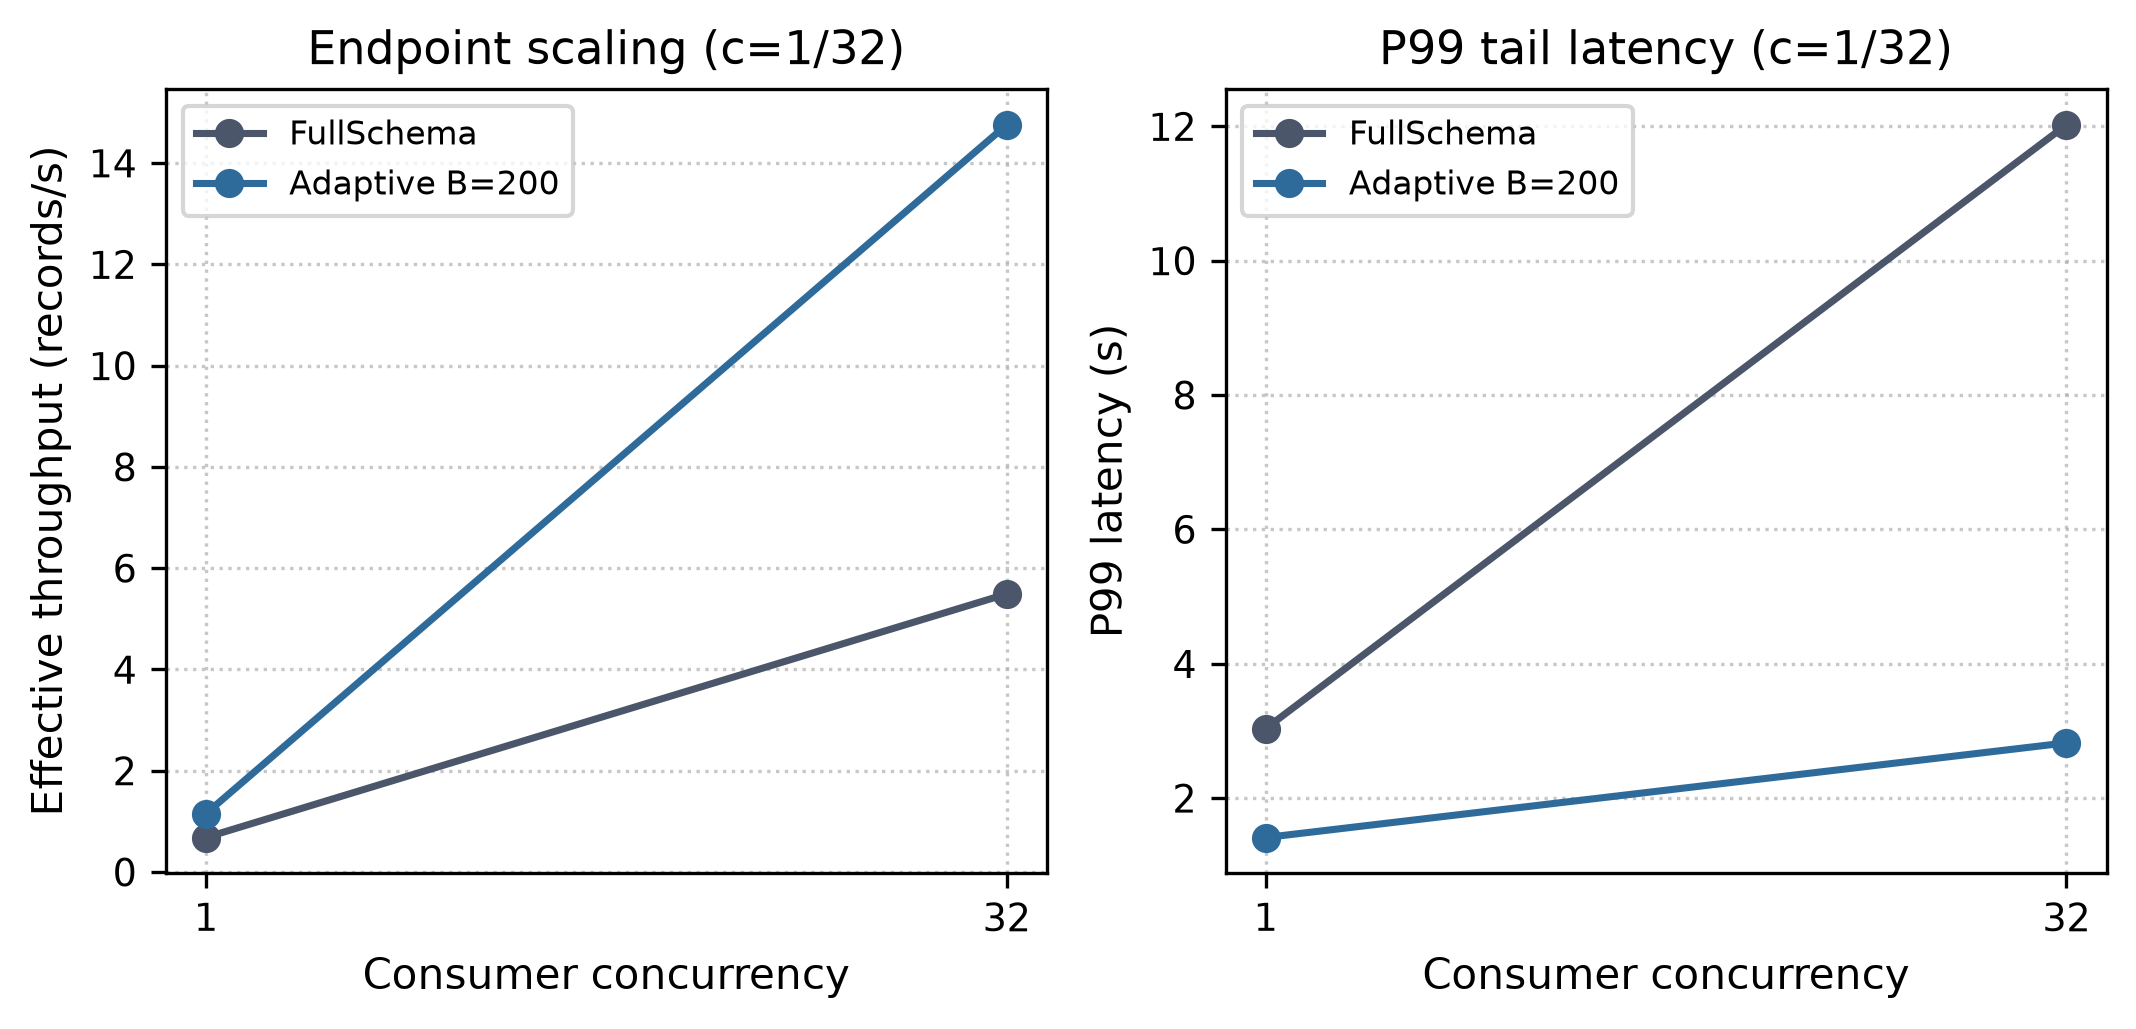
\includegraphics[width=.47\linewidth]{endpoint_scaling_and_tail_latency.png}\hfill
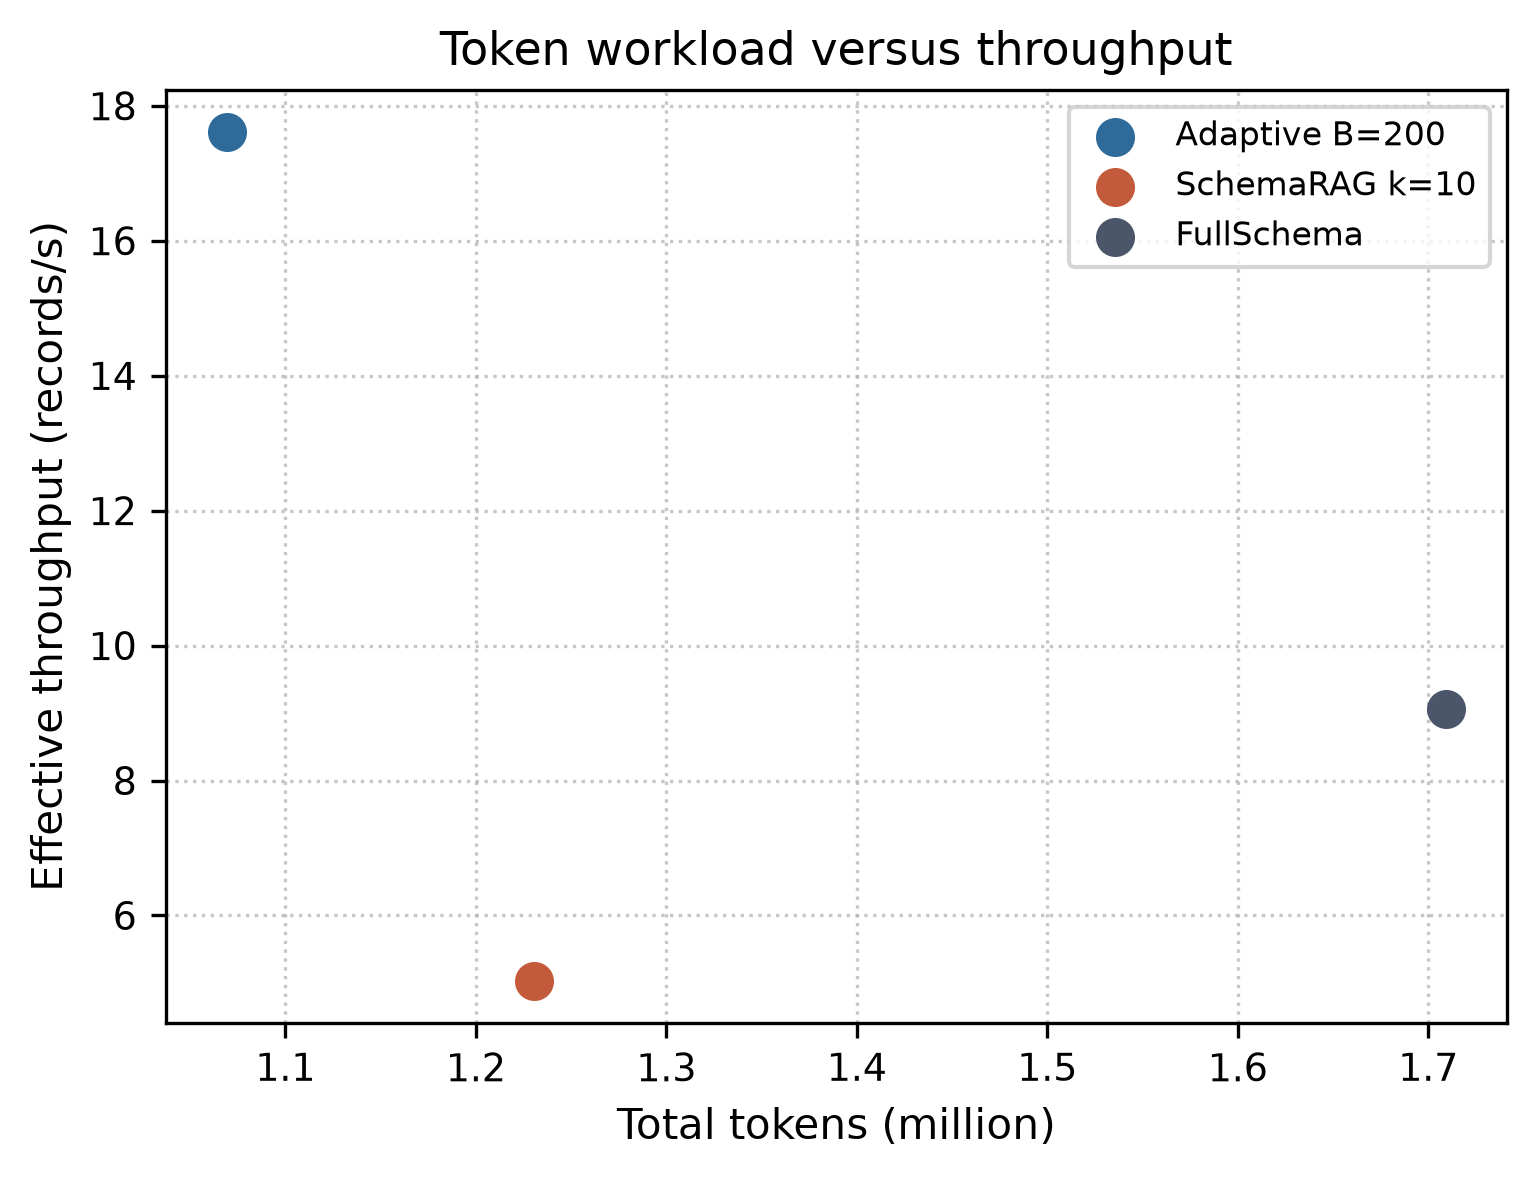
\includegraphics[width=.47\linewidth]{token_throughput_tradeoff.png}
\caption{Endpoint-direction validation and the token--throughput trade-off. The endpoint plot shows
throughput and P99 only at $c=1,q=1$ and $c=32,q=32$; it is not a full concurrency scan and cannot
separate the independent effects of concurrency and queue capacity.}
\label{fig:tradeoff}
\end{figure}

两个端点上，`budget-200` 均更快且吞吐更高，相对 `full` 的吞吐增幅分别为 68.99\% 和
168.69\%。高端点的尾延迟提示服务端排队放大；结合 SchemaRAG 的结果，系统优化不能
简化为最小化 Token，还需观察端到端时间、成功率和尾延迟。

\subsection{初始化成本边界与启动成本敏感性分析}

独立初始化实验中，100 条 M1 隔离训练三个 seed 平均耗时 737.13$\pm$43.69 ms，模型约
3.36 MB；冷加载平均 178.26$\pm$14.43 ms。100 条 FullSchema 本地规划耗时 366.63 ms
(3.09 ms/条)，按主实验速率对应的在线推理约 11.04 s，本地规划约占 3.3\%。

这些阶段不计入在线 Token 或 makespan；若需全生命周期成本，可使用：
\begin{equation}
 C_{\mathrm{amortized}}=
 \frac{C_{\mathrm{one-time\ startup}}}{N_{\mathrm{workload}}}
 + C_{\mathrm{online\ per\ record}}.
\end{equation}
当前未独立计量启动样本的外部生成成本，也不据此声称全生命周期成本降低。以已有统计
作不利的不对称换算：将训练加训练后加载的 0.915 s 只计入 `budget-200`，其时间为
114.56 s，仍低于 `full` 的 220.82 s；实际比较中两种方法共享已训练 M1，相关成本应
视为共享成本。

按主实验吞吐换算，0.915 s 和 0.178 s 分别对应约 18 条和 4 条记录的 break-even；
这仅是当前条件下的一次性成本敏感性，不适用于其他模型、硬件或并发配置。

图~\ref{fig:initialization-sensitivity} 根据主实验吞吐和已有初始化测量值作离线换算，
不是新增在线实验；0.178 s 和 0.915 s 分别对应冷加载及训练后首次加载假设。

\begin{figure}[htbp]
\centering
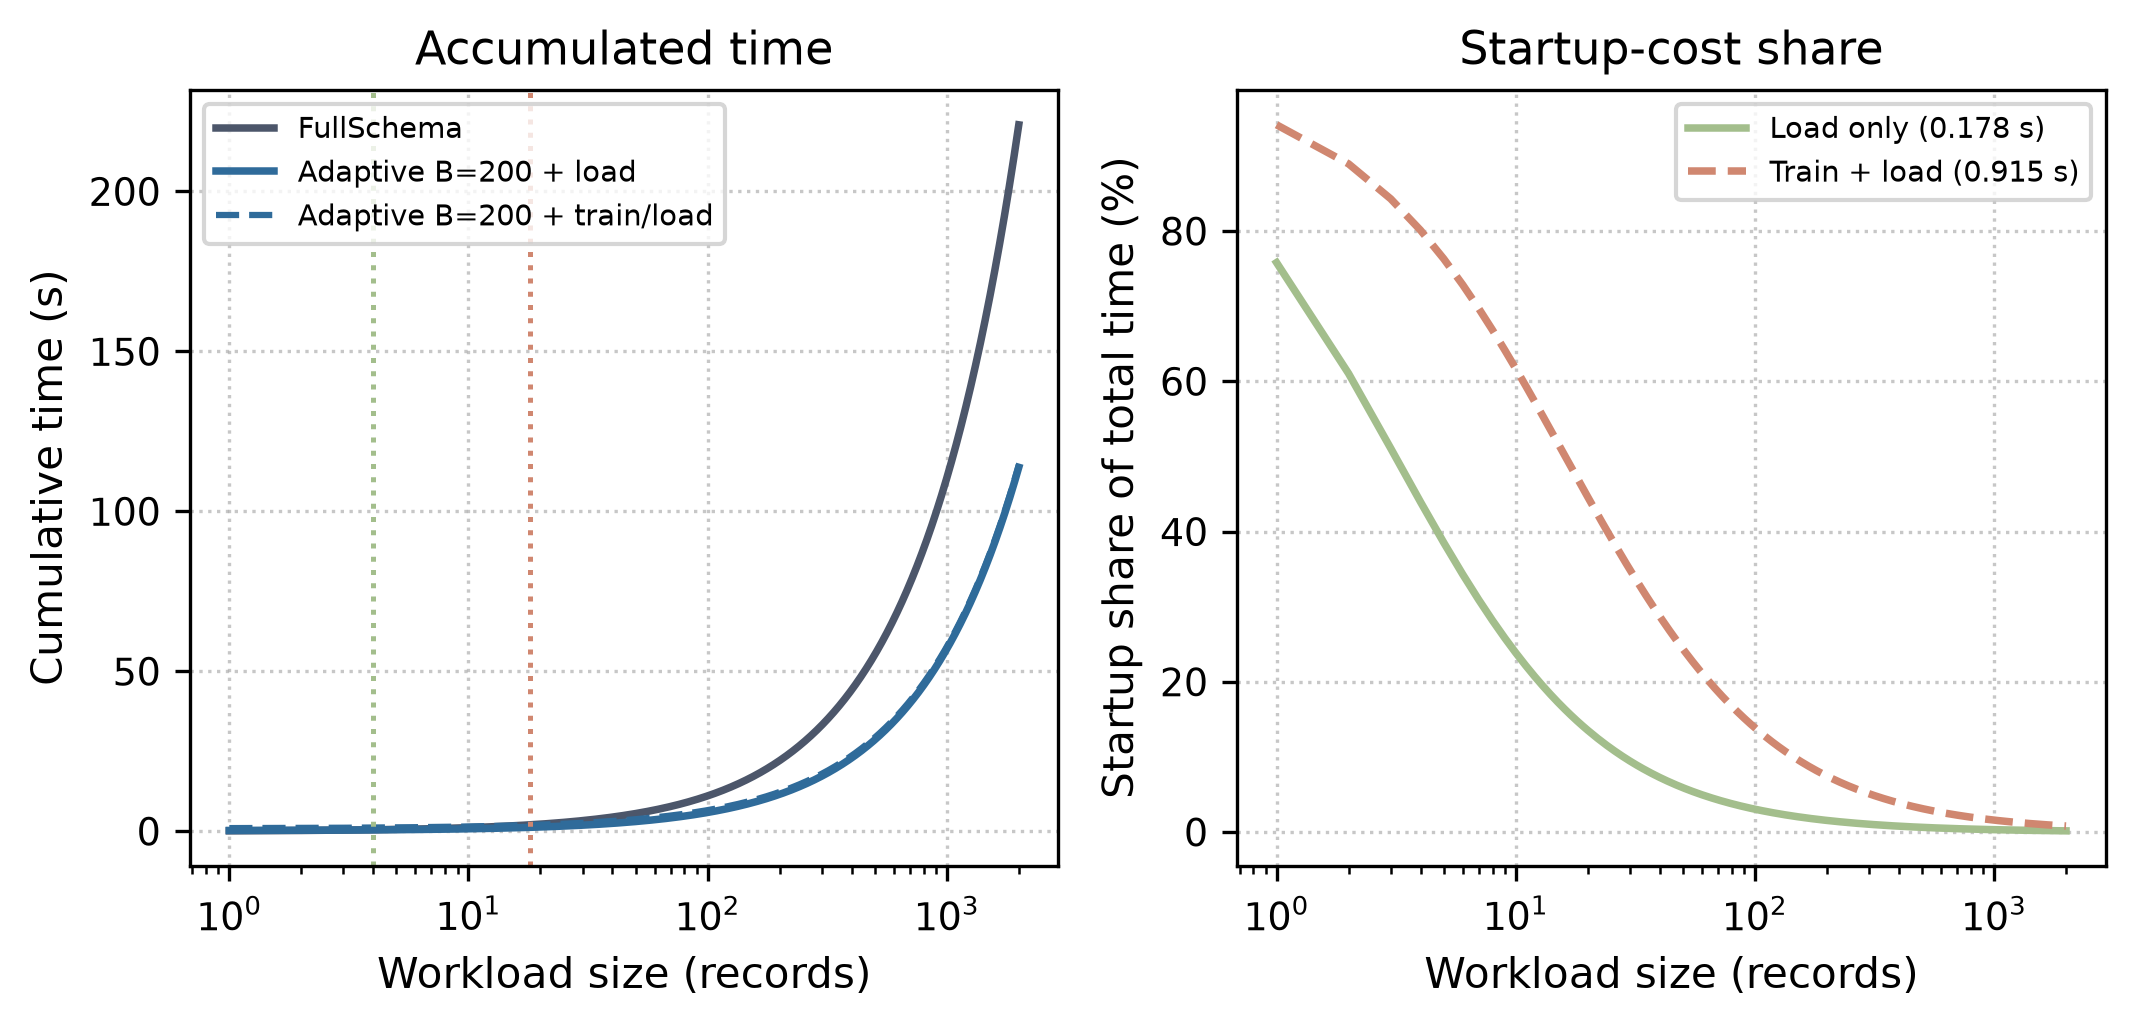
\includegraphics[width=\linewidth]{initialization_cost_sensitivity.png}
\caption{Sensitivity of the dynamic-Schema performance advantage to one-time initialization costs. Curves
are derived from main-experiment throughput and existing initialization measurements, not new online runs.
The left panel compares `full` with `budget-200` under asymmetric additions of 0.178-s cold-load and
0.915-s train-then-load costs; the right panel shows their shares of total `budget-200` time. Approximately
4 and 18 records are the corresponding break-even estimates. Both methods share the trained M1 model in
the actual comparison, so the figure does not assign these costs exclusively to the dynamic method.}
\label{fig:initialization-sensitivity}
\end{figure}

启动成本主要影响极小工作负载；随着记录数增加，在线吞吐差异成为累计时间的主要决定因素。
该分析只界定一次性成本边界，不构成完整生命周期审计。

100 条 `full` 任务的本地 Producer 规划已包含在 Runner 的在线阶段，不能重复计入；分析
不包含环境安装、容器启动、数据库冷缓存或多进程重复加载。

\section{讨论}

本文表明，少量 FullSchema 银标监督可训练出能用于真实 LLM 调用的字段选择器，但“小样本
可用”不等于对长尾字段的均衡识别。动态 Schema 在当前单进程流水线中同时降低 Token、
makespan 并提高有效吞吐；另一方面，更高覆盖率不保证更高质量，单纯减少 Schema Token
也可能被 embedding 和尾延迟开销抵消。因此评价必须联合字段质量、Token、服务时间、重试
和尾延迟。

当前结论限于以下边界：
\begin{enumerate}
  \item 监督和参考结果来自 model-assisted silver reference，不是独立人工 Gold；
  \item API 价格未配置，`actual_cost` 不是货币成本；M1 与历史 FullSchema 的不同批次
        对齐结果只能作描述性比较；
  \item SchemaRAG 是基于公开描述的外部固定 Top-$k$ 重实现，不代表官方实现；
  \item 系统为单进程异步有界流水线，性能负载为 2,000 条记录，端点同时改变 $c$ 和 $q$，
        且未验证生产规模，因而不能给出独立并发/队列因果或大规模部署结论；
  \item 在线性能不含启动样本生成、银标构造、训练和模型加载等一次性成本；敏感性分析
        仅表明当前条件下保守计入 0.915 s 不改变方向，不是完整生命周期审计。
\end{enumerate}

后续工作应补充人工或证据验证集、启动样本生成及环境和部署成本，并在固定 $c$ 下进行
$q$ 消融，再评估多进程或多节点扩展。

\section{结论}

本文提出并评估了由少量 FullSchema 银标监督驱动的预算感知动态 Schema 选择流程。M1
n=100 的 `budget-200` 在 500 条冻结记录上保持竞争性的字段指标并降低在线 Token；在
独立 2,000 条负载、16 个消费者和容量为 16 的队列条件下，流水线时间下降 48.54\%、
有效吞吐提高 94.38\%。这支持一个受限判断：对信息密度不均的记录，记录级 Schema 裁剪
可作为 LLM 预处理流水线的负载整形机制，但该判断仅适用于当前模型服务、Prompt、数据集
和单进程实现。

\section*{数据、代码与结果来源}

本文使用文化遗产记录及其派生的模型辅助银标监督。原始数据的公开范围受数据授权、
版权和隐私条件约束；本文不承诺公开受限的原始记录。数据划分、模型配置、评估报告、
派生结果和图表生成脚本将在论文发表时随附代码仓库发布，或由通讯作者在合理请求下提供。
本文中的图表均由已固化的 CSV 文件或评估报告生成；论文编译过程不发起 LLM 或 Embedding
调用。

\section*{相关工作与参考文献}

\subsection*{LLM 结构化信息抽取}
ChatSchema~\cite{chatschema}、UIE~\cite{uie} 和 InstructUIE~\cite{instructuie} 说明，
LLM 可依据预定义字段完成结构化抽取，InstructGPT~\cite{instructgpt} 代表了指令遵循能力
的发展。这类工作通常假设目标 Schema 已确定并直接提供完整字段；本文关注其调用前问题：
一条具体记录是否需要暴露全部候选字段。

\subsection*{动态 Schema 与 Schema 优化}
SchemaRAG~\cite{schemarag} 根据记录与 Schema 元数据的语义相似度检索固定 Top-$k$ 字段，
以减少上下文和输出负载。本文则用少量完整 Schema 抽取形成的模型辅助银标训练记录级
预测器，并联合字段效用、估计成本和预算约束进行选择；文中的 SchemaRAG 对照仅是公开
描述基础上的 query--field Top-$k$ 外部适配。

PARSE~\cite{parse} 优化面向 LLM 的 JSON Schema contract，Schema-adaptable Knowledge Graph
Construction~\cite{adakgc} 处理知识图谱 Schema 的全局演化；本文假设候选字段相对稳定，
研究记录级字段子集的调用前选择。

\subsection*{预算感知抽取与 Prompt 压缩}
Doctopus~\cite{doctopus} 在方案层面进行预算感知抽取，本文将决策粒度推进到记录条件下的
Schema 字段。FrugalGPT~\cite{frugalgpt} 通过路由和级联控制调用开销，LLMLingua~\cite{llmlingua}
压缩 Prompt Token；本文不改变模型或连续文本，而是在同一 LLM 服务前选择具有语义和任务
权重的字段。

\subsection*{LLM serving 与文化遗产应用}
PagedAttention~\cite{pagedattention} 从 KV-cache 管理优化 serving 吞吐；本文的
Producer--Consumer 流水线不改动服务引擎，而测量字段裁剪对请求负载、完成时间、吞吐和
尾延迟的影响，二者互为补充。Huang 等~\cite{huang2023} 提供数字文化遗产结构化管理的
应用背景；本文仅将其作为评估场景，不据此推导方法有效性、生产规模或跨数据集结论。

\bibliographystyle{splncs04}
\bibliography{references}

\end{document}
